\documentclass[a4paper, 12pt]{book}
\usepackage{graphicx}
\usepackage{textcmds}
\usepackage{subcaption}
\begin{document}
\title{Lego-LIGO User Guide \\  \large  Version 1}
\author{Dr. Chris North, Daniel Greenhouse}
\date{\today}
\maketitle

\section{Introduction}
This document is intended to provide some explanation of the workings of Lego-LIGO and its various features. The code referred  to is the python file: Lego{\textunderscore}LIGO{\textunderscore}GUI.


\section{Glossary}
\label{Glossary}
\subsection{Terms used}
Below is a description of some of the terms referred  to in both the code and this user guide.

\begin{itemize}
\item GUI is the graphical user interface displayed on the touchscreen monitor from which Lego-LIGO can be used

\item Wave-carrying beams refer to the long, moving Lego strips which the plastic waves sit on top of

\item \textit{zero} position is when the horizontal section of the wave-carrying beam \textit{is thought} to lie between the two rows of red tiles on the floor of Lego-LIGO

\item \textit{hard zero} position is when the horizontal section of the wave-carrying beam \textit{actually} lies between the two rows of red tiles on the floor of Lego-LIGO

\item Degrees refers to the degrees that the motor has moved through. Due to the design of the motor mechanism this is directly proportional to the displacement of the mirror from the \textit{zero} position

\item \q{Manual} and \q{Self-Movement} are analogous

\item \q{Preset} and \q{Choose a Movement} are analogous

\item Motor A is mirror X

\item Motor B is mirror Y

\item A \textit{normal} button in calibration and manual mode is either \q{Forward} or \q{Backward}

\item A \textit{fast} button in calibration and manual mode is either \q{Fast Forward} or \q{Fast Rewind}

\end{itemize}

\subsection{Button functions}
The following buttons perform the said functions throughout.

Home, figure \ref{fig:Home Button}, returns to the home screen shown in figure \ref{fig:Home Screen}

Exit, figure \ref{fig:Exit Button}, exits the application

Next, figure \ref{fig:Next Button}, loads the next screen of the GUI

\begin{figure}[ht]
\centering
\begin{subfigure}{.25\textwidth}
\centering

\includegraphics[width=25mm]{Home_Button.png}
\caption{Home Button}
\label{fig:Home Button}
\end{subfigure}
\begin{subfigure}{.25\textwidth}
\centering

\includegraphics[width=25mm]{Exit_Button.png}
\caption{Exit Button}
\label{fig:Exit Button}
\end{subfigure}
\begin{subfigure}{.25\textwidth}
\centering
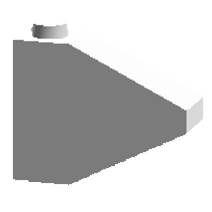
\includegraphics[width=25mm]{Next_Button.png}
\caption{Next Button}
\label{fig:Next Button}
\end{subfigure}
\caption{Images of buttons used throughout the GUI.}
\end{figure}


\section{Understanding the motors and the mirror's movements}
\label{motor section}
\subsection{How the mirrors move}
Each motor can be told at what power\footnote{\label{power meaning}The power output is in the python file: BrickPi. The input has no discernable units and so power and speed can be seen as the same in this situation.} it should run at. The mirrors move as a consequence of an inputted motor power and inputted time that the motor should run for in sections 13 or 14 of the code; section 13 calculates these whereas section 14 has them inputted from previous functions. The code makes use of python's timer by taking the current time when the motor command is called and then running the motor at the inputted power while the difference between the current time and the time that the motor command is called is less than the inputted time. Then, while the time difference is greater than the inputted time but less than the sum of the inputted time and the so called \q{stop{\textunderscore}buffer}, the motor is run at zero power. This gives the motor time to stop at its current position rather than allowing the motor to \textit{coast} past its desired position.

This method appears to work adequately but is by no means precise and is a source of the constant need for calibration. Should the user encounter issues with the stopping time of the motor they may wish to alter \q{stop{\textunderscore}buffer} in section 3 \textit{PARAMS} of the code. Also in section 3 \textit{PARAMS} is \q{pwrcoef} which is the coefficient for translating power to the motor degree position. This is measured from the motor itself and may need to be altered should the user see fit.


\subsection{How the position of the mirrors is tracked}
One of the biggest difficulties the user shall encounter when using Lego-LIGO is the discrepancy between the actual motor position and the assumed motor position. As previously mentioned, the degree position of the motor is directly proportional to the displacement of the mirror (providing it stays on the rack) and so guessing the motor's degree position shall suffice.

The motors cannot provide direct feedback to the BrickPi and so it is up to section 11 of the code (\q{position{\textunderscore}tracker}) to guess at the position of the motor. Whenever there is a command to move the motor, in sections 13 and 14, the power that each motor runs at and the time that each motor runs for is passed into the \q{position{\textunderscore}tracker}. This updates the global parameters \textit{MXPos} (motor X position) and \textit{MYPos} (motor Y position) according to the equation

$\textit{motor power}\times\textit{time the motor runs for}\times\textit{the power coefficient}$.


\section{Getting Started}
The Raspberry Pi will turn on when power is supplied to it. It requires, at least\footnote{\label{power cables}Both the monitor and the Raspberry Pi can take a miniUSB, but the power is shared and so two power cables can power all three.}, two power cables; one power cable\footnote{\label{BrickPi power cable}Type: at least 600mA; 12V; exterior diameter is 5.5mm; interior diameter is 2.5mm} should go to the Brick Pi and a miniUSB should go to either the touchscreen monitor or the Raspberry Pi. If insufficient power is being supplied to the Pi a yellow lightning bolt shall appear in the top-right corner of the screen.

On start up please double click on the \q{runLegoLIGO} application which is available on the desktop. An \q{Execute File} window shall load and the user should select \q{Execute}. The GUI shall load.


\chapter{Using Lego-LIGO}
\section{Welcome Screen}
On start up the GUI shall display the \q{Welcome Screen} as shown in figure \ref{fig:Welcome Screen}. The cross in the top right of the screen exits the application. The arrow in the bottom right proceeds to the \q{Calibration Screen} as shown in figure \ref{fig:Calibration Mode Screen}.
\begin{figure}[ht]
\centering
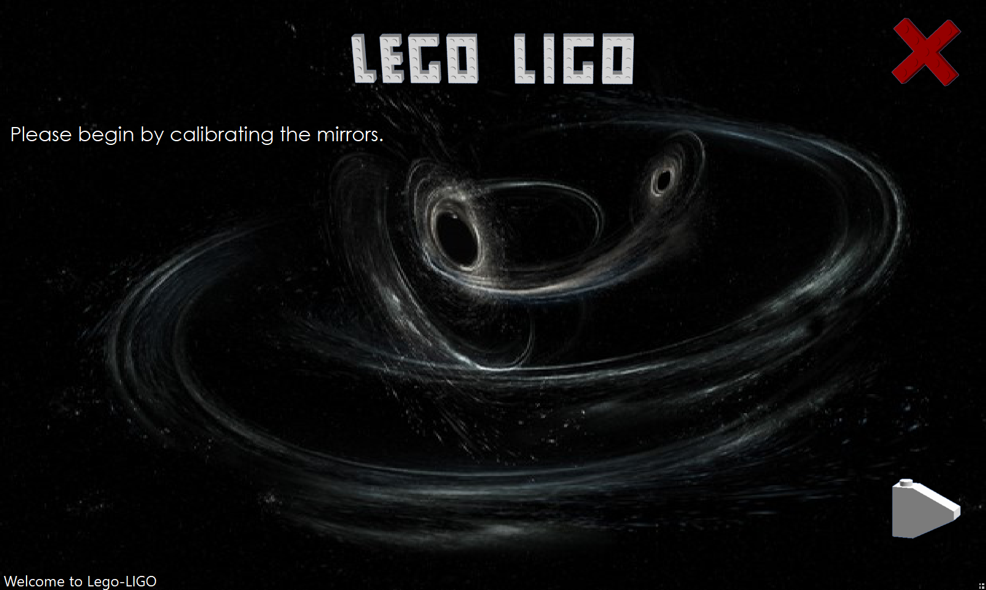
\includegraphics[width=120mm]{Welcome_Screen.png}
\caption{Welcome Screen}
\label{fig:Welcome Screen}
\end{figure}



\section{Calibration}
The calibration mode allows the user to move the mirrors back and forth using the buttons provided. It is shown in figure \ref{fig:Calibration Mode Screen}. The \textit{fast} buttons move the mirrors quicker and longer by factors specified in section 3  \textit{PARAMS} of the code\footnote{For more information, see section \ref{software edits} of this document}. The user should use the motor controls to move the front, wave carrying arms until the cross beam lies between the rows of red tiles. This is specified in the on-screen instructions.

The user should then select the \q{set calibration} button which is the white tick (in the bottom right-hand corner of figure \ref{fig:Calibration Mode Screen}, second in from the right). To encourage the user to do so, the home button shall only appear once the \q{set calibration} has been pressed.

This sets the global parameters \textit{MXPos} and \textit{MYPos} to be at 0. It is worth noting that this is a very approximate tracking system since it relies on where the motors should be rather than on feedback from the motor as to where they actually are. As a consequence the motors should be regularly calibrated.
\begin{figure}[ht]
\centering
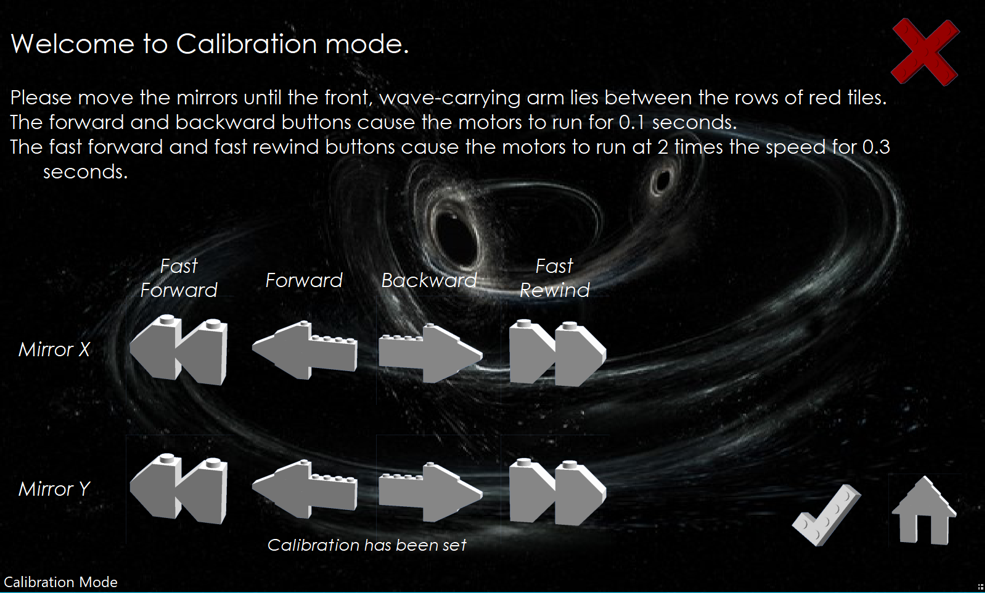
\includegraphics[width=120mm]{Calibration_Screen.png}
\caption{Calibration Mode Screen}
\label{fig:Calibration Mode Screen}
\end{figure}


\section{Home Screen}
The \q{Home} screen is loaded whenever the home button (shown in figure \ref{fig:Home Button}) is pressed. It is shown in figure \ref{fig:Home Screen}.

The \q{Home} screen provides the user with three options: \q{Calibration}, \q{Manual}, and \q{Preset}. Selecting these shall load the subsequent screen (Calibration is the same as before).

On selection of \q{Preset} the mirrors shall return to their \textit{zero} position. This is based on the tracked position and so may be slightly different to the \textit{hard zero} position.
\begin{figure}[ht]
\centering
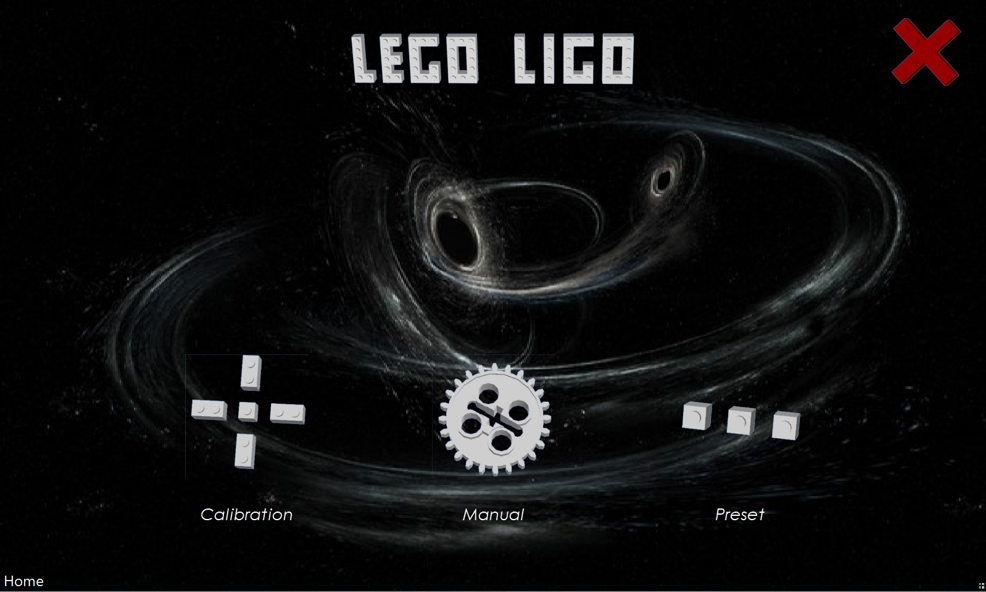
\includegraphics[width=120mm]{Home_Screen.png}
\caption{Home Screen}
\label{fig:Home Screen}
\end{figure}


\section{Manual}
In \q{Manual} mode the user is presented with the same motor movement types as in \q{Calibration} mode. It is shown in figure \ref{fig:Manual Mode Screen}.

Manual mode is to be used for when the demonstrator wants control of the motors. This can be particularly useful for explaining interference.

The key difference between \q{Manual} and \q{Calibration} mode is that paramaters in section 3 \textit{PARAMS}\footnote{\label{manual/calibration scaling} see section \ref{software edits} of this document} scales/alters the time and power run at. The idea behind this is to make \q{Manual} mode easier when explaining the interference.

When the motor has moved too far from the \textit{zero} position (also specified in section 3 \textit{PARAMS}\footnote{\label{manual limit} see section \ref{software edits} of this document}), a message shall display on the screen and the mirrors shall return to their \textit{zero} position. This is to prevent the user from continuously running the motor past its limit which could cause damage to Lego-LIGO.

On exit the mirrors shall return to their \textit{zero} position. This is based on the tracked position and so may be slightly different to the \textit{hard zero} position.
\begin{figure}[ht]
\centering
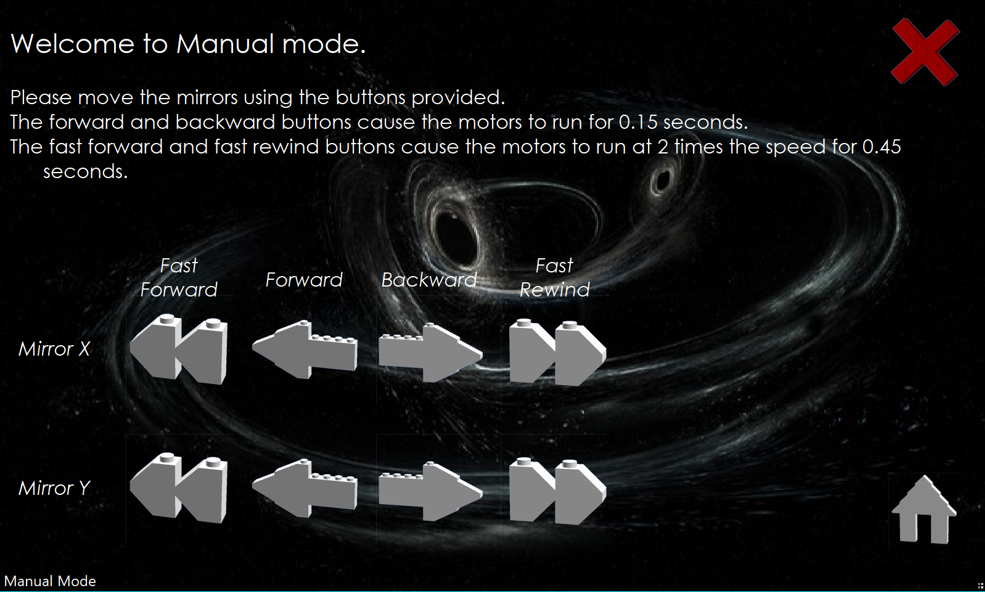
\includegraphics[width=120mm]{Manual_Screen.png}
\caption{Manual Mode Screen}
\label{fig:Manual Mode Screen}
\end{figure}

\section{Preset}
The \q{Preset} mode offers the user a list of movements. It is shown in figure \ref{fig:Preset Mode Screen}. These are the names of the \q{.csv} files in the \q{Test code} folder.

Before selecting a movement the user should take particular care to ensure that the motors are close to their \textit{hard zero} position\footnote{\label{zero discrepency}There is some margin of error given by \q{presetbuffer}, see section \ref{software edits} of this document}.

The screen has a maximum limit of 10 files and adding more \q{.csv} files to the \q{Test code} folder shall load the \q{File Warning} screen shown in figure \ref{fig:File Warning Screen}.

Choosing a file shall load the corresponding \q{Graph} screen.
\begin{figure}[ht]
\centering
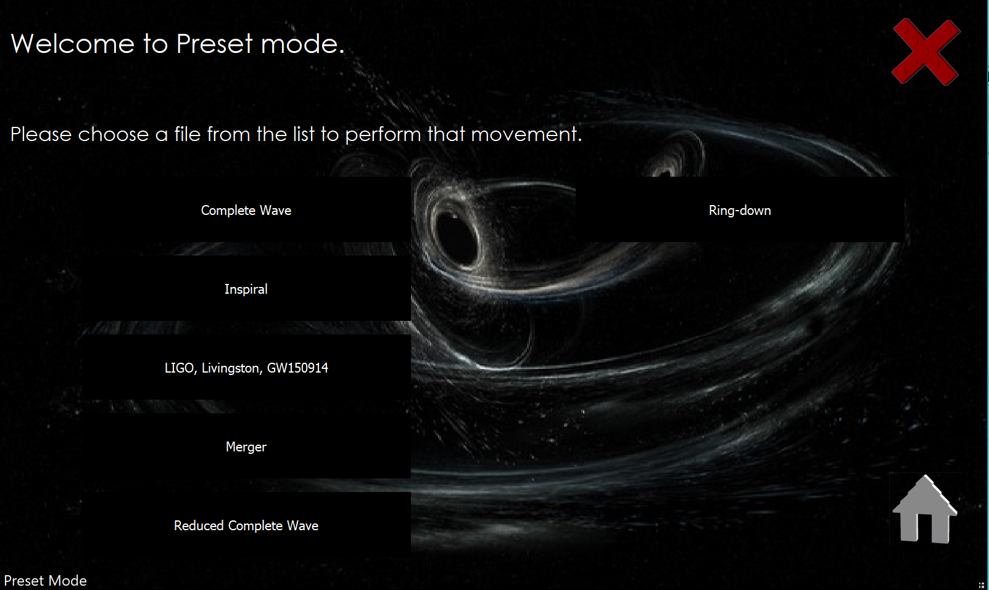
\includegraphics[width=120mm]{Preset_Screen.png}
\caption{Preset Mode Screen}
\label{fig:Preset Mode Screen}
\end{figure}


\section{Graph}
Once a movement has been selected from the options in \q{Preset} mode, the GUI shall display the graph of the selected movement. An example of this is shown in figure \ref{fig:Graph Screen}. The graph has strain on the y-axis. This uses a rough approximation of the change in mirror position and the length of one of Lego-LIGO's arms. Should the user want to find this accurately they should alter \q{strain} in section 6 of the code. Time is on the x-axis.

It is here also that the motors receive their commands to move.

The user must wait until the motors have finished performing their selected movement and then returned to their \textit{zero} position. The status bar shall alert the user when the mirrors are returning to their \textit{zero} position.

Once finished, the user should press the \q{Home} button located in the bottom-right corner of the screen to return to the \q{Home} screen.
\begin{figure}[ht]
\centering
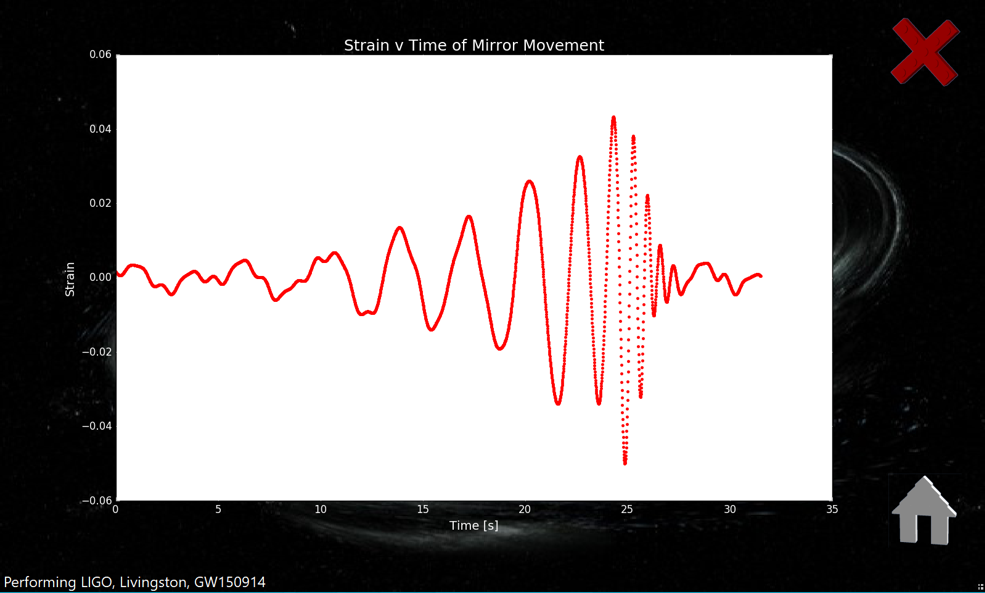
\includegraphics[width=120mm]{Graph_Screen.png}
\caption{Graph Screen}
\label{fig:Graph Screen}
\end{figure}

\section{File Warning}
When more than 10 files are in the \q{Test Code} folder, the screen shown in figure \ref{fig:File Warning Screen} shall be displayed when \q{Preset} is chosen from the \q{Home} screen.

This is due to insufficient space on the screen. See section \ref{Adding files} of this document for more information.
\begin{figure}[ht]
\centering
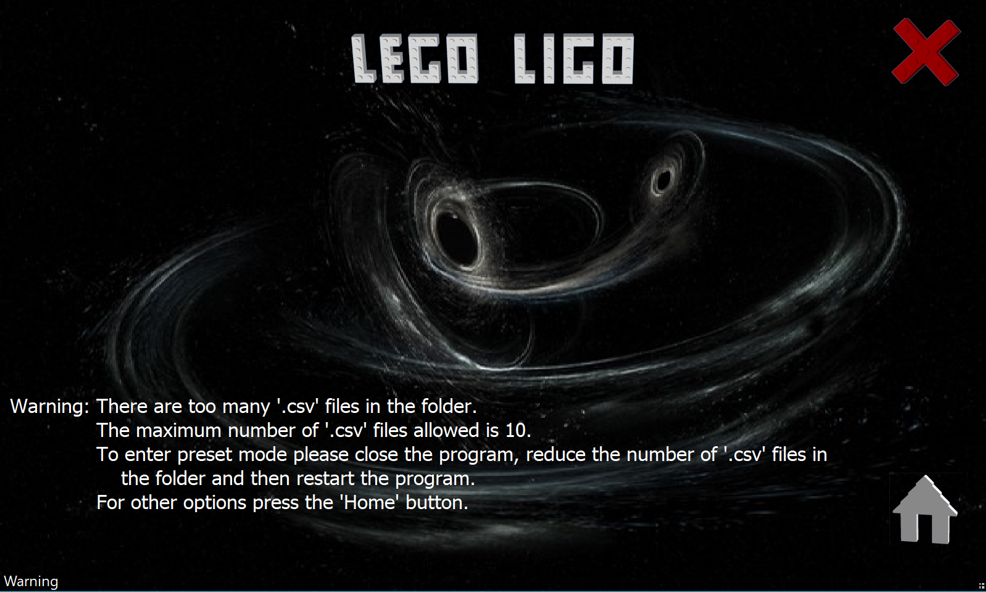
\includegraphics[width=120mm]{File_Warning_Screen.png}
\caption{File Warning Screen}
\label{fig:File Warning Screen}
\end{figure}

\section{Speed Warning}
The screen shown in figure \ref{fig:Motor Warning Screen} shall be displayed if a file is chosen from the \q{Preset} screen that contains a gap between data points which would require the motor to run at an unachievable speed.\footnote{\label{speed warning note}n.b. currently this is not working when in \q{Stationary Point} mode. For further information see sections \ref{Motor Modes} and \ref{Future Edits} of this document.}

This limiting speed is set manually in section 6 and should be investigated by checking the limit of motors used.
\begin{figure}[ht]
\centering
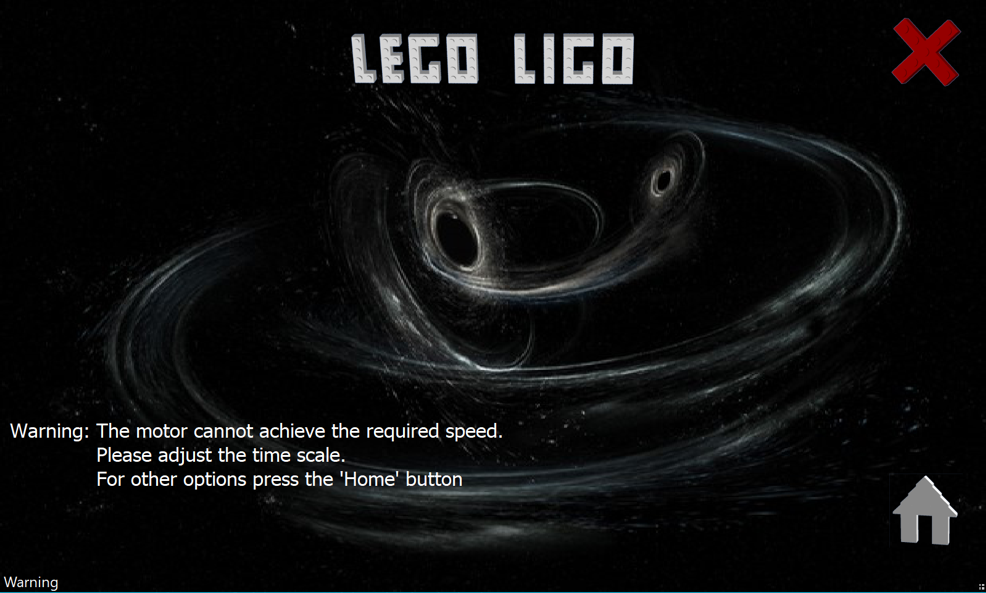
\includegraphics[width=120mm]{Motor_Warning_Screen.png}
\caption{Motor Warning Screen}
\label{fig:Motor Warning Screen}
\end{figure}


\chapter{Editing Lego-LIGO}
When wishing to edit Lego-LIGO on a PC different to the Raspberry Pi, the user should make the following adjustments to the code:
\begin{itemize}
\item in section 1 of the code, the \q{RP} toggle should be set to \q{False}
\item in section 3 of the code, a valid file path of the file containing the images should be entered in \q{else: IMAGE{\textunderscore}LOCATION =}
\item in section 3 \textit{PARAMS} of the code, a valid file path of the \q{Test Code} file containing all of the \q{.csv} files should be entered in \q{FOLDER}
\end{itemize}
The user may wish to also alter the window dimensions in section 7 of the code under \q{else}.\footnote{\label{RP monitor change}RP is True should be left intact unless the touchscreen monitor is to be replaced}

\section{Motor Modes}
\label{Motor Modes}
Lego-LIGO can recreate the waveform using the motors in two ways. One finds the stationary points of a wave and runs the motor to these points. The other selects the data point every x\footnote{\label{data point spacing}x is the data point spacing and can be specified in section 3 \textit{PARAMS} \q{data{\textunderscore}point{\textunderscore}spacing}, for more information see section \ref{software edits} of this document} seconds. Some waveforms may work better in one mode or the other although most tend to work better when finding the stationary points since this limits the motor's \textit{jerky} movements.

The \q{Stationary{\textunderscore}points =} toggle allows the user to choose between these modes. \q{True} makes the motors run to each stationary point while \q{False} makes the motors run to the data point at every x seconds.


\section{Adding Files}
\label{Adding files}
Lego-LIGO can take on additional preset movements. Should the user wish to add additonal preset movements they should do so by taking the file and saving it in the designated \q{Test Code} folder. The file should be of \q{.csv} type and have two columns of first time and second strain. The time is scaled by the amount stated in section 3 \textit{PARAMS}, \q{time{\textunderscore}scale}. The strain is relative since when the motor performs the file it takes the maximum strain difference and then corresponds this to the maximum number of degrees that the motor can turn through. It is assumed that the first line of the file is the column heading and so this line is skipped when the file is read.

A maximum of ten files are allowed in the \q{Test Code} folder, exceeding this limit shall bring up the \q{File Warning} screen, shown in figure \ref{fig:File Warning Screen}, when the \q{Preset} mode is selected from the \q{Home} screen shown in figure \ref{fig:Home Screen}.


\section{Images}
Should the user wish to change an image, the following convention is used.
\begin{center}
\begin{tabular}{ c c c }
 Use & Name & Type \\
\hline
 Background Image & Background & JPG \\  
 Title Image & Title & PNG \\
 Home Button Image & Home & PNG \\
 Exit Button Image & Exit & PNG \\
 Calibration Button Image & Calibration & PNG \\
 Manual Button Image & Manual & PNG \\
 Preset Button Image & Preset & PNG \\
 Next Button Image & Next & PNG \\
 Set Calibration Button Image & Set & PNG \\
 Fast Forward Button Image & Fast{\textunderscore}Forward & PNG \\
 Forward Button Image & Forward & PNG \\
 Backward Button Image & Backward & PNG \\
 Fast Rewind Button Image & Fast{\textunderscore}Rewind & PNG
\end{tabular}
\end{center}

\section{GUI}
In sections 8 and 9 of the code there is a system for the positioning of buttons and labels. These all scale with the window dimensions and some sections require x and/or y positions when there are several similar buttons to position them accordingly on the screen. If the user wishes to alter these they should read the comments in the various subsections of the code in order to gain understanding of the positioning (it should be fairly self-explanatory from the names of the variables). Sections 8 and 9 do not create the buttons or labels (these are created in user interface setup in section 15) but instead just alter the appearance.

\section{Troubleshooting}
\subsection{Software}
\label{software edits}
The user may find it beneficial to read through section \ref{motor section} of this document before deciding to make any alterations that they see necessary.

The following are descriptions of some of the quick edits that the user may wish to make by making use of the parameters in section 3 \textit{PARAMS} of the code. Terms from the glossary, section \ref{Glossary}, are used.

\begin{description}
\item [Overall Maximum Degree.] To change the maximum degree that the motor can run to from zero, alter \q{degree{\textunderscore}max}. This should be a direct measurement of the degrees turned through from the \textit{hard zero} position and the limit of Lego-LIGO.

\item [Preset Maximum Degree.] To change the maximum degree that the motor can run to while in preset mode, alter \q{presetbuffer}. This multiplies the previously mentioned maximum degree by the given amount ( \q{presetbuffer}) and so changing the maximum degree shall also affect the distance the mirrors move in preset mode. This shall only affect the preset movement and is especially useful when determining the wavelength etched onto the plastic strips. It helps to ensure that the mirrors don't \textit{crash} and so by using a lower buffer value the user can perform more preset movements between calibrations before the discrepancy between actual motor position and assumed motor position causes a \textit{crash}.

\item [Manual Maximum Degree.] To change the maximum degree that the motor can run to while in manual mode, alter \q{manualbuffer}. This multiplies the previously mentioned maximum degree by the given amount (\q{manualbuffer}) and so changing the maximum degree shall also affect the maximum distance the mirrors can move in manual mode. This shall only affect the manual movement and is used to help prevent the user from \textit{crashing} the mirrors. Once the limit has been reached the mirrors shall immediately return to their \textit{zero} position.

\item [Mirror Return Speed.] To change the speed of the mirrors when returning to their \textit{zero} position, alter \q{return{\textunderscore}pwr}.

\item [Manual, \textit{Normal} Speed.] To change the speed of the mirrors when a \textit{normal} button in manual mode is pressed, alter \q{self{\textunderscore}movement{\textunderscore}pwr}.

\item [Calibration, \textit{Normal} Speed.] To change the speed of the mirrors when a \textit{normal} button in calibration mode is pressed, alter \q{Calibrate{\textunderscore}pwr}.

\item [Calibration and Manual, \textit{Fast} Speed.] To change the speed of the \textit{fast} buttons relative to the \textit{normal} buttons in calibration and manual mode, alter \q{Fast{\textunderscore}power{\textunderscore}multiplier}. This simply multiplies the power given to the motor when the \textit{standard} buttons are pressed by the said amount (\q{Fast{\textunderscore}power{\textunderscore}multiplier}) to give the power given to the motor when the \textit{fast} buttons are pressed.

\item [Time Scale.] To change the time multiplier from the \q{.csv} file to that performed by the motors, alter \q{time{\textunderscore}scale}.

\item [Manual, \textit{Normal} Time.] To change the time that the motors run for with each press of a \textit{normal} button in manual mode, alter \q{self{\textunderscore}movement{\textunderscore}run{\textunderscore}time}.

\item [Calibration, \textit{Normal} Time.] To change the time that the motors run for with each press of a \textit{normal} button in calibration mode, alter \q{Calibrate{\textunderscore}run{\textunderscore}time}.

\item [Calibration and Manual, \textit{Fast} Time.] To change the time that the \textit{fast} buttons cause the motors to run for relative to the \textit{normal} buttons in calibration and manual mode, alter \q{Fast{\textunderscore}time{\textunderscore}multiplier}. This simply multiplies the time that the motors run for when the \textit{standard} buttons are pressed by the said amount (\q{Fast{\textunderscore}time{\textunderscore}multiplier}) to give the time that the motors run for when the \textit{fast} buttons are pressed.

\item [Power coefficient] To change the power coefficient when translating power and time to degree position, alter \q{pwrcoef}.
\end{description}

\subsection{Hardware}
Lego-LIGO's main vulnerability is the dislodging of the wave-carrying beam and mirror from the motor. Should the motors run past their limit the mirror's rack and wave-carrying beam's rack could run off the motor's cog. This should be fixed by entering calibration mode\footnote{manual mode could be used but typically calibration mode uses smaller mirror movements with each press and shall not cause the mirrors to reset their positions once degree max has been reached}. The user should run the motor forward until both sets of racks come completely off the cogs. There can be difficulty detaching the wave-carrying beam and this should be dealt with by carefully raising it above any hardware limits. Do not worry if the beam breaks since it is easier to repair this once the racks return under the cogs influence. Mirror X causes extra difficulty due to the corner mechanism. Depending on the severity of the separation, the user may find it useful to remove the shortest wave-carrying beam.

The user should begin by rejoining the mirror. The user should ensure the mirror's racks are square to the motor and slowly push it toward the motor until it reaches the cogs. While keeping a slight pressure on the mirror toward the motor, run the motor backward using the \q{backward} button. Once the mirror has a good few pins past the cog, the user should attach the wave-carrying beam. This should be done in the same manner, paying particular attention to ensuring the racks are square to the motor. Once the mirror and wave-carrying beam is re-attached, the user should check a successful operation by running the mirror back and forth. The hardware limits should be felt by the wave-carrying beam only. If the mirror interferes with this the user should start again.

Finally, with mirror X only, the user should run the mirror to its forward limit. Once there, the user should replace the shortest wave-carrying arm at its own limit (up against the outer wall) ensuring it fits correctly in the groove. It is sensible to again check the hardware stops are felt by the long, wave-carrying beam only.

For other issues with the breakage of parts of the Lego the computer model\footnote{This is the Lego Digital Designer LXF Model File (.lxf), entitled \q{Lego-LIGO Model}} should be consulted. This has a complete replication of Lego-LIGO although over time designs may change slightly from it and certain Lego parts may become unavailable. Consequently, the user should use their own discretion in the rebuild.

For the more vulnerable parts, such as the mirror cases and around the motor enclosure, gluing should be considered.

A Raspberry Pi 3 is used with a Dexter Industries modified Raspbian OS stored on a micro SD card. A Dexter Industries BrickPi + hat is used alongside Lego Mindstorms Large motors. The monitor is \q{The Official Raspberry Pi 7" Touchscreen} with a 800 x 480 pixel display.

\section{Furture Edits}
\label{Future Edits}
Future users may wish to provide the following edits:
\begin{itemize}
\item fix the bug in the resetting
\item Add a stop button to the preset movement
\item Plot the graph as the motor is moving.
\item Provide a motor speed warning when the motor is in stationary points mode
\item Change the plastic wave strips with sinusoidal waves etched on for \textit{opacity gradient} waves and make use of Lego's Light sensor and an LED to provide real-time feedback of the interference.
\end{itemize}


\chapter{Contacts}
For any further queries please feel free to contact:

Daniel Greenhouse

University of Birmingham

dmg697@student.bham.ac.uk
\end{document}